\subsection{Impact of batch size on validation accuracy}
\label{subsection:experiments:classification:batch}
Although the batch size seems unimportant in comparison with neural network architecture and the choice of an optimizer, the experimental data from Figure \ref{figure:experiments:classification:batch-size-plot} indicates that the batch size plays an important role when the network is trained for a fixed number of iterations. To examine the effects of various batch sizes, a reasonably large neural network architecture is chosen and such a network is trained using the configuration from Table \ref{table:expriments:training_config}. In this experiment, only the batch size and activation function are varied. It is very important to note that the number of epochs remained unchanged. 

The results displayed in Figure \ref{figure:experiments:classification:batch-size-plot} indicate that training using smaller batch sizes results in significantly greater validation accuracy. This can be attributed to the fact that a smaller batch size implies a greater number of parameter updates since the number of epochs is fixed. It is worth noting that such a training setup requires significantly more time. For instance, the average training time using a batch size of 32 examples was about 30 minutes, while the average training time using the batch size of 256 examples was about 5 minutes. The accuracy drop after the batch size of 128 is noticeable for every activation function. This could be expected since the number of parameter updates drops significantly. On the other hand, a larger batch size often results in a more accurate estimate of the gradient.

It seems that larger batch sizes generally require a larger number of training epochs, which is indeed sensible, as the optimization performs significantly less parameter updates. It is reasonable to conjecture that the sweet spot for the default training configuration is a batch size of 64 examples, as it seems that such a configuration performs slightly better than other batch sizes in 2 out of 3 activation functions.

To sum up, batch size likely plays an important role in training a neural network. The results discussed are relevant only for one neural network architecture and one default training setup. However, according to the Figure 1 from \cite{hoffer_2018_train} and Figure 2 from \cite{shirishkeskar_2017_on}, the similar observations can be made on more complex datasets and neural networks. It is interesting to note that \cite{hoffer_2018_train} and \cite{shirishkeskar_2017_on} provide different explanations and analysis of this phenomenon.

\begin{figure}[H]
    \centering
    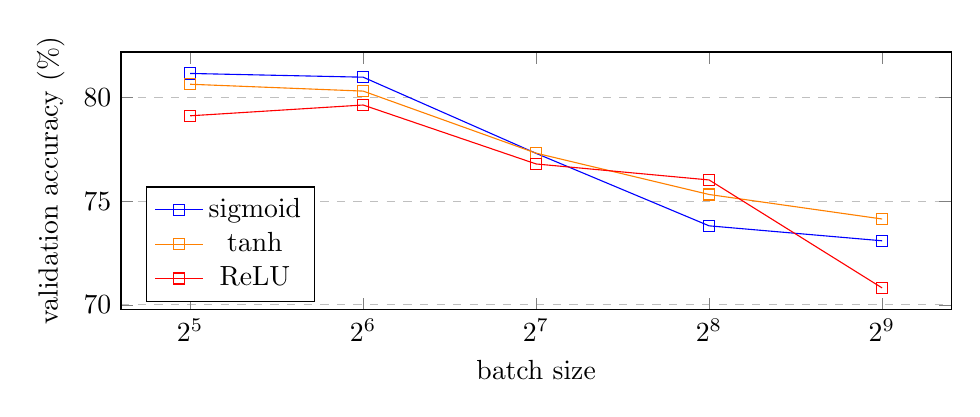
\begin{tikzpicture}
        \begin{axis}[
            height=0.4\textwidth,
            width=\textwidth,
            xlabel={batch size},
            ylabel={validation accuracy (\%)},
            ymajorgrids=true,
            grid style=dashed,
            xmode=log,
            legend pos=south west,
            log basis x={2}]
            \addplot[mark=square,blue] coordinates {(32,81.15) (64,80.97) (128,77.30) (256,73.81) (512,73.09)};
            \addplot[mark=square,orange] coordinates {(32,80.63) (64,80.30) (128,77.31) (256,75.32) (512,74.14)};
            \addplot[mark=square,red] coordinates {(32,79.11) (64,79.63) (128,76.79) (256,76.02) (512,70.82)};
            \legend{sigmoid, tanh, ReLU}
        \end{axis}
    \end{tikzpicture}
    \caption{Effects of various batch sizes on training \textit{nn-2x-128-sigmoid-softmax}}
    \label{figure:experiments:classification:batch-size-plot}
\end{figure}